\chapter{Optimized Path Planning} \label{chap:trial}
\iffalse
Keywords : 
Smooth Tour Construction with kinematic constrains,Dubins TSP,
Bezier Curve , cubic spline interpolation

bezier curve:
% http://www.joics.com/publishedpapers/2011_8_12_2441_2450.pdf

http://www.ijsce.org/attachments/File/v3i2/B1421053213.pdf
good explanation but it doesnt formulate as TSP . so refer to the book of planning and motion of UAV.


Global planner, local planner can be found  in lecture 10 planning of visual navigation for flying robots .. slide 79 before and after
The approach provided in this thesis is 2 layers of path planning. The first one is the global path planning where  the waypoints are sorted based on the shortest distance covered traversing all the given waypoints. The second layer is finding the paths between intermediate waypoints. 
This second layer can
\fi

As mentioned earlier in the previous chapter, the best waypoints to be traversed guaranteeing area coverage were chosen. Path planning algorithm should be implemented afterward to sort these waypoints in order to assure minimal traversal 3D euclidean distance. After sorting the waypoints, there are several methods to achieve the trajectory planning that the robot should follow in between them.

These processes of sorting the waypoints, then traversing in-between them;  can be formally explained as 2 layer path planning consisting of; global and local planners. Autonomous navigation of an aerial robot based on the combination of evolutionary algorithms as a global planner. Followed by one choice of the approaches discussed in section \ref{local_path_planning} as a local planner. These approaches can be summed up as a linear piecewise function, spline piecewise function and artificial potential fields.


% The hybrid approach first uses Grid Method where the robot environment is represented by orderly numbered grids, each of which represents a location in the environment. Then, it applies Genetic Algorithm (GA), a global planner, to find an optimal path according to the current environment. The GA proposed here uses an evolutionary population initialization and genetic operators, which make the evolutionary process converge after some populations. Finally, a new Artificial Potential Field method, a local planner, is applied to follow the path obtained by GA from one intermediate node to next intermediate node avoiding the obstacles. Experimental results clearly illustrate that the proposed hybrid approach works well on large scale dynamic environments.


%\textcolor{red} { hybrid PF with GA, 
%http://download.springer.com/static/pdf/746/chp%253A10.1007%252F978-94-007-2792-2_31.pdf?originUrl=http%3A%2F%2Flink.springer.com%2Fchapter%2F10.1007%2F978-94-007-2792-2_31&token2=exp=1463649025~acl=%2Fstatic%2Fpdf%2F746%2Fchp%25253A10.1007%25252F978-94-007-2792-2_31.pdf%3ForiginUrl%3Dhttp%253A%252F%252Flink.springer.com%252Fchapter%252F10.1007%252F978-94-007-2792-2_31*~hmac=ec049bb412555489f79488635013bb217387263b0f56bf6ea86e6e0965c82648
%}


Normally path planning optimization techniques does not put the constraint of passing by the defined waypoints as a hard constraint in their solutions. But rather, tend to change the waypoints depending on the robot motion in relative to the environment. In this thesis's case hard constrains of passing by the waypoins are taken into account. A global path planner is good in producing a minimal distance path, but poor in finding intermediate waypoints and reacting to unknown obstacle.

%\textcolor{red}{rectilinear environment}
%so we can not rely on cell decomposition % page 7 paper carera 

\section{Global Path Planning } \label{global_path_planning}
There are several ways to globally solve and find the robot path within a map. % lazem te3mel 7esab el map di hatnail fiha eh !! 

%formulate this problem. In this Thesis, two methods have been implemented and compared.

Some operations research methods, such as traveling salesman problem (TSP), Chinese postman problem and rural postman problem can be considered. In this thesis; TSP was taken into account. 


\subsection{Problem Formulation}


% The list of waypoints needs now to be sorted to compute an efficient path with smoother shape and shorter traveling distance. 

% \iffalse
% A process of using Dijkstra to compute an ordered list of waypoints providing shorter path. These waypoints in the sorted list is dealt with as temporary goals for the UAV to pass through. The next step is to fit the trajectory of the UAV as in \cite{curve_path}. For this waypoints are dealt as if they are graph nodes and transform the problem to be a linear or spline piecewise function .  
% \fi
% A process of formulating the problem of shortest path as traveling sales man problem and finding optimized solution using genetic algorithm is approached previously many times \textcolor{red}{citation} and validated its working principle, so it is used here in this context. The path output as ordered list of poses that guarantee the shortest path. The next step is to fit the trajectory of the UAV as in \cite{curve_path}. For this waypoints are dealt as if they are graph nodes and transform the problem to be a linear or spline piecewise function.


\subsubsection{Search Based Shortest Path Problem}
The goal of this category of methods is to find a continuous curve (no need to be smooth) in a configuration space that begins from the start node $x_{init}$ to the goal end node $x_{goal}$. It is mature enough method in research field with several algorithms like Dijkstra, A*, D*, and many more. % as discussed in the background 

%In our case we assume every waypoint as a goal, which define the problem as multi-goal Dijkstra path planning problem. The robot will search within its neighbour nodes for the node generating shortest path to every goal.
Representing the waypoints chosen previously as a weighted graph. The nodes of the graph are the waypoints, vertexes are an intermediate path between waypoints. The weights of the vertices are the Euclidean distances between waypoints. Dijkstra is then implemented to find the minimum cost path.

 %Dijkstra in this method will simply find at every iteration the waypoint with the shortest euclidean distance from the current waypoint. Traversed waypoint will be excluded at every iteration. At the end of this process a list of ranked waypoints with the least 3D euclidean distance between every waypoint and its succedent one is obtained. This will not guarantee a globally shortest distance path.
 Iteratively, Dijkstra will start from the initial node and search within the connected nodes for the one with the least weight. Choose this node to be its next initial node and repeat the process till all the required nodes are traversed and ranked.

%\textcolor{red}{write in algo Sora kaman momken}

%transform the area to be covered to a graph % transform the area to grid with discretize the graph up to a resolution needed  assign each pose as a node in the graph assign 3D Euclidean distance as the weight of the vertex between the nodes.

It is wide known of its slowness in the topological representation. The resolution and amount of waypoints considered as goals lead to very slow and nonoptimal convergence for passing by all these waypoints, so another formulation is required to be tested. The formulation discussed in the next section shows promising results.

\subsubsection{Traveling Sales Man Problem }
The robot traversing the waypoints can be formulated as traveling sales man problem(TSP). The TSP can be shortly explained as a salesman has to visit several cities (or road junctions). The goal is to find the salesman's route of minimum length with the constrain of passing by by all the cities only once. Mathematically modeling the problem as a complete graph with n vertices, the salesman will make a tour or hamiltonian cycle  \cite{dantzig1954solution}.

Sorting the path can be addressed as an optimization problem. Every node which is a point in space (3D position) is represented as a city and the euclidean distances between the cities are calculated and used as the optimization cost function. The path is organized based on the minimum length of traversing over all the waypoints. To find an optimized solution GA is used. The privilege of TSP problem formulation and solving it using GA over the other shortest path algorithms like Dijkstra, is that it provides global complete solution traversing all the waypoints not finding a path from a starting node to a goal node. The GA approach for multiple waypoint path planning is more clarified and discussed by Trevor \textit{et al.} in \cite{davies2006multiple}.


GAs generally consist of three operators: selection, crossover, and mutation. The evaluation function for the N cities two-dimensional Euclidean TSP is the sum of Euclidean distances between every pair of cities in the tour. 

That is: 
\[Cost function = \sum_{i=1}^{N}  \sqrt{(x_{i}-x_{i-1})^{2}+(y_{i}-y_{i-1})^{2}} \]
                                           
Where, $x_{i}$, $y_{i}$  are the coordinates of city i and  $x_{N}$, $y_{N}$   equals $x_{0}$, $y_{0}$. %We also make some changes to the encoding, selection, and recombination.

The algorithm can be explained in abstract as :
%\textcolor{red}{|||||||||||||||||}

%1. Generate a new population of the previous population by updating all paths in the current population. The point hereditary is determined. The path is amended by deleting the initial points and adding other segments to reach all paths to the end point.\\
%2. Start the algorithm for a static planning to the population and find the best path.\\
%3. Send the best path to the aerial robot when it reached the crossing point current.\\
%4. Update estimates of site locations for the environment.\\
%5. Go back to step one.\\

% REF : https://www.cs.indiana.edu/~vgucht/Genetic_Algorithms_for_the_Travelling_Salesman+Problem.pdf
% http://www.obitko.com/tutorials/genetic-algorithms/tsp-example.php
% http://www.ijsce.org/attachments/File/v3i2/B1514053213.pdf
%Algorithm 2 Genetic Algorithm

%1. Start
%2. Population initialization
%3. Repeat until satisfying stop criteria
%4. Selection
%5. Cross-over: two selected chromosomes can be combined by a cross-over operator, the result of which will replace the lowest fitness chromosome in the population. Selection of each chromosome is performed by an algorithm to ensure that the selection probability is proportional to the fitness of the chromosome. A new chromosome has the chance to be better than the replaced one. The process is oriented towards the sub-regions of the search space, where an optimal solution is supposed to exist.
%6. Mutation: a gene from the selected chromosome is randomly changed. This provides additional chances of entering unexplored sub-regions. Finally, the evolution is stopped when either the goal is reached or a maximum CPU time is reached.
%7. Making new population with the fittest solutions
%8. Evaluation
%9. Checking the stop criteria
%10. Take the best solution as output
%11. End

% http://www.lalena.com/AI/Tsp/
% http://www.theprojectspot.com/tutorial-post/applying-a-genetic-algorithm-to-the-travelling-salesman-problem/5

\begin{enumerate}
\item Create a group of many random tours in what is called a population. This algorithm uses a greedy initial population that gives preference to linking cities that are close to each other.
\item Pick two of the shortest tours which represent better parents in the population and combine them to make 2 new child tours. Hopefully, these children tour will be better than either parent.
\item A small percentage of the time, the child tours are mutated. Mutation of a tour is done by multiple ways like shuffling or swapping the route. Shuffling the route is done by randomly moving one of the cities from one point in the tour to another. Mutation is done to prevent all tours in the population from looking identical.
\item Crossover is done by picking two parents. Then take subset from the first parent and complete the child formation from the second parent.
\item The new children tours are inserted into the population replacing a number of the longest tours. The size of the population remains the same in every generation.
\item New children tours are repeatedly created until the desired goal is reached.
\end{enumerate} 


%\textcolor{red}{see the 3 dimentional part !! change in the code to adapt and then change the passage }



%B. The Algorithm GA
%1. randomly initialize population(t)
%2. determine fitness of population(t)
%3. repeat
%  1. select parents from population(t)
%  2. perform crossover on parents creating
%  population(t+1)
%  3. perform mutation of population(t+1)
%  4. determine fitness of population(t+1)
%4. until best individual is good enough 
%
%\begin{algorithm}
%\caption{}\label{alg:euclid}
%\begin{algorithmic}[1]
%\Procedure{N}{$a$}
% \State $S\gets 0$
%  \While{$eval Cost(S)\leq ThresholdRate$}
%	 \State $S \gets GA(NWayPoint)$
%	  \State $NWayPoint\gets NWayPoint+1$
%  \EndWhile\label{endwhile}
%\State \textbf{return} $NWayPoint$
%\EndProcedure
%\end{algorithmic}
%\end{algorithm}



% The privilege of GA over the Geometric Algorithms and sampling based algorithms is finding a complete solution traversing all the waypoints not finding a path from a starting node(pose) to a goal node(pose) %, not like grid or probabilistic methods used to navigate from one waypoint to another

% After having a sorted list of poses to be traversed, the next step is to fit the trajectory of the UAV as in Chang et al \cite{curve_path}.
\vfill

\begin{figure}[!h]
\minipage{0.53\textwidth}
  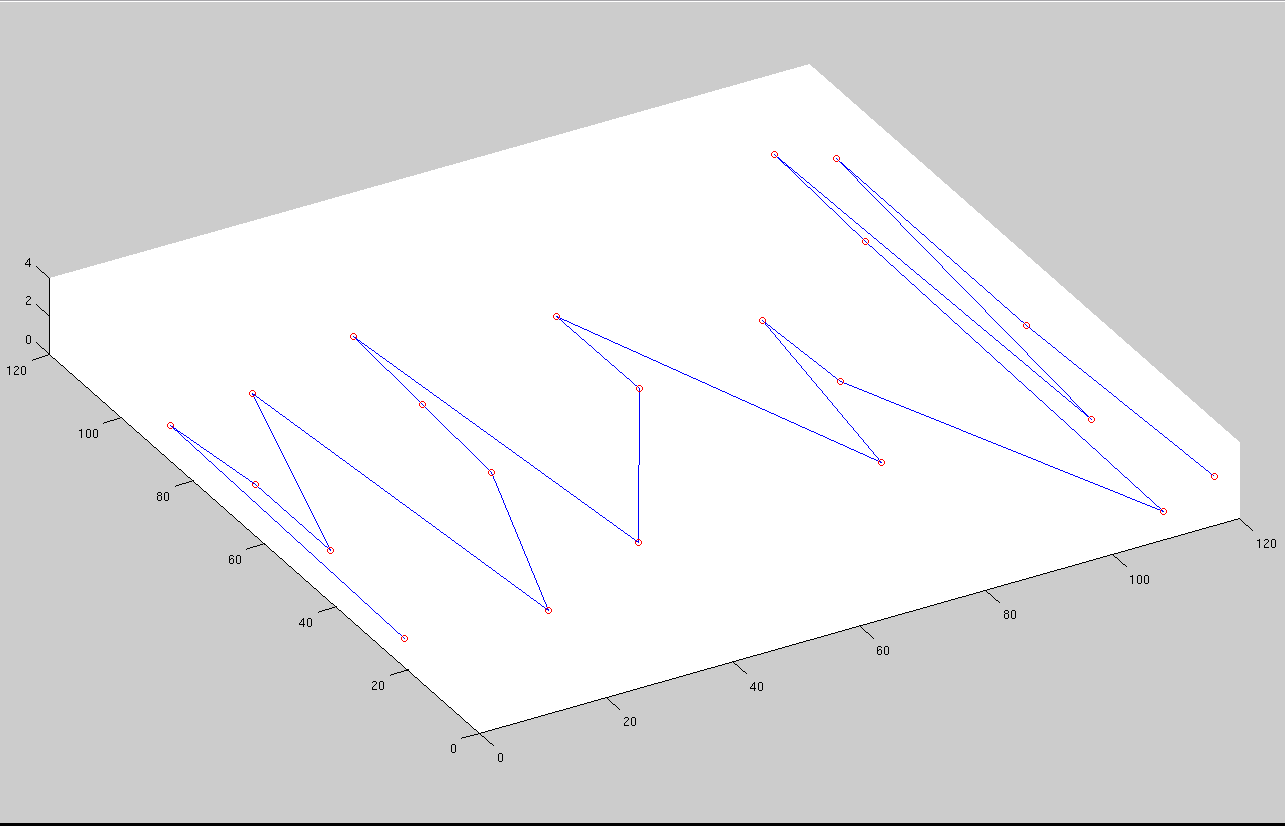
\includegraphics[width=\linewidth]{figures/DijkstraPath2.png}  
  \endminipage\hfill
  \minipage{0.45\textwidth}
   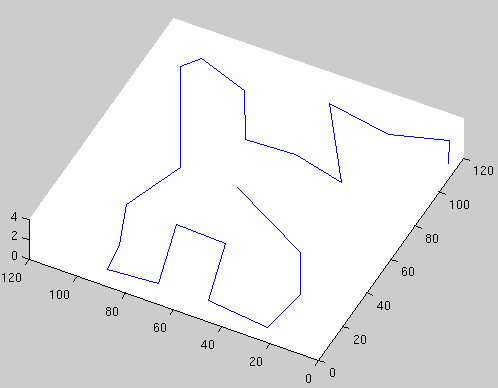
\includegraphics[width=\linewidth]{figures/Path_planned_G.png}
  \caption{Path using Dijkstra vs GA}
  \label{fig:Path_planning}
  
  \endminipage 
\end{figure}

%Traversing Distance was shorten by the 3.2 factor.  Before the path planning the distance traversed  was 166 meters and after GA applied it is nearly 51.3 meters 

The distance covered by a path that is planned by GA is 513 meters which is shorter by the factor of 1.8 compared to the distance covered by Dijsktra multi-goal approach which is 963 meters.


\section{Local Path Planning} \label{local_path_planning}

After succeeding in getting the main waypoints sorted in a way to grantee shortest path length. Forthwith comes the issue of generating the mid waypoints that the robot should traverse to generate the trajectory.

Three main ways have been implemented and tested. These ways will be mentioned in the next three subsections.

\subsection{Linear Piecewise Interpolation}
The previous process will provide a list of sorted  waypoints co-ordinates. These waypoints are dealt as graph nodes, that need to be connected to have a path, so the problem is formulated as a linear or spline piecewise function.

 Hereby the used linear piecewise function used in Eq.(\ref{eq:3}).

\begin{equation} \label{eq:3}
f(x)=
\left\lbrace
\begin{array}{ccc}
0  & \mbox{if} & x\leq a\\
\frac{x-a}{b-a} & \mbox{if} & a\leq x\leq b \\
\frac{c-x}{c-b} & \mbox{if} & b\leq x\leq c \\
1  & \mbox{if} & c\leq  x \\
\end{array}\right.  ,
\end{equation}

\noindent 
Where the line segment between points \textit{a} and \textit{b} will be the line between every waypoint and the consecutive one. The third point is \textit{c} and depending on the number of waypoints variables will be added in the formula. Discretizing this point up to an extent will act as the sampling the path. % to form a trajectory.


% \textcolor{red}{Shall i write the general equations of linear and spline piecewise fn. ?!}
% \textcolor{davidS}{????? i thing is more about ingeniery and implementation on robots }



\subsection{Spline Piecewise interpolation }
% for the equation : https://en.wikipedia.org/wiki/Spline_interpolation


% REF : http://www.math.colostate.edu/~gerhard/classes/331/lab/splines.html
% http://www.sciencedirect.com/science/article/pii/0736584589900458

% VERY IMPORTANT TO SIMPLIFY : http://citeseerx.ist.psu.edu/viewdoc/download?doi=10.1.1.713.6275&rep=rep1&type=pdf

% Field D*: http://robots.stanford.edu/isrr-papers/final/final-23.pdf

% https://www.youtube.com/watch?v=YtcZXlKbDJY

%spline length is shorter than polynomial interpolant

 The goal of the spline interpolation is to find the shortest smooth path through consecutive waypoints. This smoothness is advisable in order to eliminate the sudden change in the first derivative or the slope of the function (the line between the waypoints). It is very important as, robots specially aerial ones, require a portion of time and space to change direction and rotate. 
 
% Moreover, the discontinouity in the fist derivative of the poses (velocities); which are used in the low level control of the robot's motors .

% ‘spline’ - not-a-knot cubic spline interpolation

%length of the interpolant = \textcolor{red}{there is a way to calculate it check }

When the interpolation is assumed to be piecewise linear, it is relatively easy. However, if the curve is to be a spline, perhaps interpolated as a function of chordal arc length between the points, this gets a bit more difficult. A nice trick is to formulate the problem in terms of differential equations that describe the path along the curve. Then the interpolation can be done using an ordinary differential equation solver. For instance, the robot used in this thesis is a quadcopter; which is considered to be holonomic. Its kinematics give hovering capabilities. This feature permits to relax turning constraints on the path (which represents a crucial problem for fixed-wing vehicles).
The implemented interpolation as shown in the results section \ref{experiment_reuslts} is a cubic spline. This cubic spline of the $i^{th}$ spline function, in general, can be written as:
\begin{equation}
s_{i}(x)=a_{i}+b_{i}(x-x_{i})+c_{i}(x-x_{i})^2+d_{i}(x-x_{i})^3
\end{equation}
For n data points, there are n-1 intervals and thus 4(n-1) unknowns to evaluate to solve all the spline function coefficients. $a_{i}$, $b_{i}$, $c_{i}$, and $d_{i}$ must be determined for each \textit{i}. More investigation about spline interpolated path planning can be found in \cite{judd2001spline}.

% https://www.math.ohiou.edu/courses/math3600/lecture19.pdf

\subsection{Artificial Potential Field}
It was promising idea when Artificial Potential Field (APF) was first introduced in the robotics field by Oussama Khatib in 1986 \cite{khatib1986real}. With simple rules defined in the paper as a potential function between free space and obstacle space. The goal position to be reached is an attractive pole for the robot and obstacles are repulsive surfaces.

% stated The manipulator moves in a field of forces \textcolor{red}{explain more}. 

The procedure involves the following steps:
\begin{enumerate}
\item Establish a potential field function.
\item Locate a minimum potential point using any optimization algorithm.
\item Navigate an object toward the minimum potential point.
\item Repeat steps 2 and 3 until the object reaches the goal position.
\end{enumerate}

\begin{equation}
\begin{split}
U(q)=U_{att}(q)+U_{rep}(q) \\
U_{rep}(q)=\sum(U_{obstacles}(q))
\end{split}
\end{equation}

\begin{equation}
F(q)=-\nabla U(q)
\end{equation}
Where
$U_{att}$ is the attractive potential and
$U_{rep}$ is the repulsive potential. F(q) is the local force that will let the robot move by small steps.
There are various functions to model the potential field. The parabolic one is used in this context. 
Following an iterative gradient decent can be a simple way to go to the bottom where the goal point is available. 

\[q_{i+1}=q_{i}+\delta_{i}\frac{F(q)}{\left \| F(q) \right \|}\]


% online collision avoidance approach

As obstacle avoidance was the original goal of this algorithm, potential fields come with the risk of getting stuck in local minima and not being able to reach the goal. There are several solutions to this inherent characteristic. one of them is to methods like RRT to plan the path in the generated potential field map like what stated by Latombe et al. in \cite{latombe2012robot,planningBook}. In our specific case, the global path planner set the initial point and the goal point provided to the APF with a guarantee to have a short distance which should not lead to a local minimum. Here APF is tweaked to only avoid the obstacles that may appear in the map, not planning the whole path.
% parameters like the rotation and .... blbla has to be defined for the robot to navigate the whole map.
\section{Summary}

%\textcolor{red}{ the pathplanning book 3.5.2.2 GA PF}

\begin{figure}[H]

  \includegraphics[width=0.92\textwidth]{figures/main(1).png}
  \caption{Pipeline of the methodology}
  
  \label{fig:pipeline_1}  
\end{figure}